% \textbf{Title: Sampling 1}

Consider a signal with this spectrum.

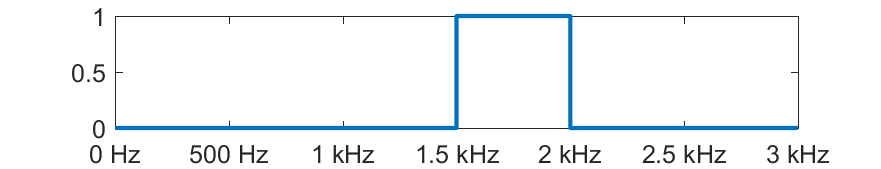
\includegraphics[width=4.60233in,height=0.88285in]{../../Images/SamplingAndAliasingQ1.png}

How can we choose the sampling frequency \(f_{s}\) if we want to reconstruct the original signal with an ideal low-pass filter? \\

a. \(f_{s} = 1.5\ kHz\).

%@ Incorrect. This question tests the concept ``Sampling and Aliasing'', which is taught in these courses.

b. \(f_{s} = 2.9\ kHz\).

%@ Incorrect. This question tests the concept ``Sampling and Aliasing'', which is taught in these courses.

c. \(f_{s} = 3.5\ kHz\).

%@ Incorrect. This question tests the concept ``Sampling and Aliasing'', which is taught in these courses.

*d. \(f_{s} = 4.1\ kHz\).

%@ Correct! This question tests the concept ``Sampling and Aliasing'', which is taught in these courses.

e. I do not know. \\

%@ It's okay. This question tests the concept ``Sampling and Aliasing'', which is taught in these courses.
